\documentclass[10pt]{article}
\usepackage{icmlko}

\icmlmeta{IP 파운데이션 월드모델}{295}{가려던 자리가 더 거친 자리였다}{세 노트에서 ``하네스는 분해능이 다르다''고 전제하고 갈 곳으로 적었다 --- 재 보니 lab 보다 일곱에서 서른 배 거칠다}

\begin{document}

\twocolumn[
\icmlheader

\begin{abstract}
노트 291 · 293 · 294가 전부 ``남은 것''의 첫 줄에 \textbf{하네스에서 재기 ---
MAPE 쪽은 분해능이 다른 유일한 자리}를 적었다. 세 번 적는 동안 \textbf{한
번도 안 쟀다.} 쟀다. 하네스에는 이미 짝 A/B 셋(시장층 · 피처 · 신호, 서로
레코드가 안 겹치는 30 · 29 · 27건)과 반복 실행 로그가 디스크에 있다. 노트
274의 법칙(검출 문턱 ${=}$ 2$\times$짝SE)을 그대로 적용했다. \textbf{지표
수준으로 정규화한 문턱이 lab 은 2$\sim$10\% 인데 하네스는 15$\sim$65\% 다}
--- 일곱에서 서른 배 \textbf{거칠다.} 그리고 실측 라벨을 쓰는 내부 폴드가
\textbf{제일 거칠다}(65\%) --- 내가 계속 인용하던 ``MAPE 16$\sim$18\%''가
바로 그 폴드다. 원인은 표본이다: lab 은 유보 2,675행을 채점하고 하네스는
A/B 당 27$\sim$30건이다. \textbf{그래서 하네스가 지금까지 보고한 세 개선이
전부 자기 문턱 아래다}($t{=}0.52 \cdot 1.07 \cdot 1.74$). 여기서 멈추지 않고
갈랐다(노트 133) --- APE 는 \emph{이미 비율}이라 차보다 \textbf{비}가 맞는
척도다. 배수 척도로 다시 재니 셋이 \textbf{$t{=}1.64 \cdot 1.58 \cdot 1.51$
로 거의 같고} 방향도 같다. 서로 안 겹치는 세 셋을 합치면
$n{=}86$ · \textbf{$t{=}+2.69$} · 주입이 APE 를 \textbf{21.4\% 줄인다}. 다중비교
$m{=}4$ 기준 2.50은 넘고 $m{=}8$ 기준 2.73은 \textbf{못 넘는다.}
그리고 각 셋에 필요한 표본이 \textbf{45$\sim$47건}인데 지금 27$\sim$30건이고
\textbf{안 쓴 라벨이 120건 남아 있다.} \textbf{갈 곳이 아니라 넓힐 곳이었다.}
\end{abstract}
]

\section{세 번 적고 한 번도 안 쟀다}

노트 291 · 293 · 294의 ``남은 것'' 표가 전부 같은 줄로 시작한다.

\begin{center}\small
\begin{tabular}{ll}
\hline
노트 & 적은 것 \\
\hline
291 & 하네스에서 재기 --- 분해능이 다르다 \\
293 & 하네스에서 재기 --- 분해능이 다른 유일한 자리 \\
294 & 하네스에서 재기 --- MAPE 쪽은 분해능이 다르다 \\
\hline
\end{tabular}
\end{center}

``다르다''고 썼지만 \textbf{쓴 뜻은 `더 낫다'}였다 --- lab 에서 잰 것이 전부
문턱 아래로 끝나니 문턱이 낮은 데로 가자는 뜻이었다. 그건 \textbf{측정이
아니라 희망}이다. 잴 재료는 이미 디스크에 있었다.

\begin{center}\small
\begin{tabular}{lrl}
\hline
짝 A/B & $n$ & 무엇을 뺐나 \\
\hline
\texttt{market-eval-v3} & 30 & 시장 층 \\
\texttt{feat-eval} & 29 & 피처 \\
\texttt{sig-eval} & 27 & 신호 \\
\hline
\texttt{runvar} & 9$\times$4 & --- (같은 팔 반복) \\
\hline
\end{tabular}
\end{center}

세 셋은 \textbf{레코드가 하나도 안 겹친다.}

\section{일곱에서 서른 배 거칠다}

\begin{figure*}[t]
\centering
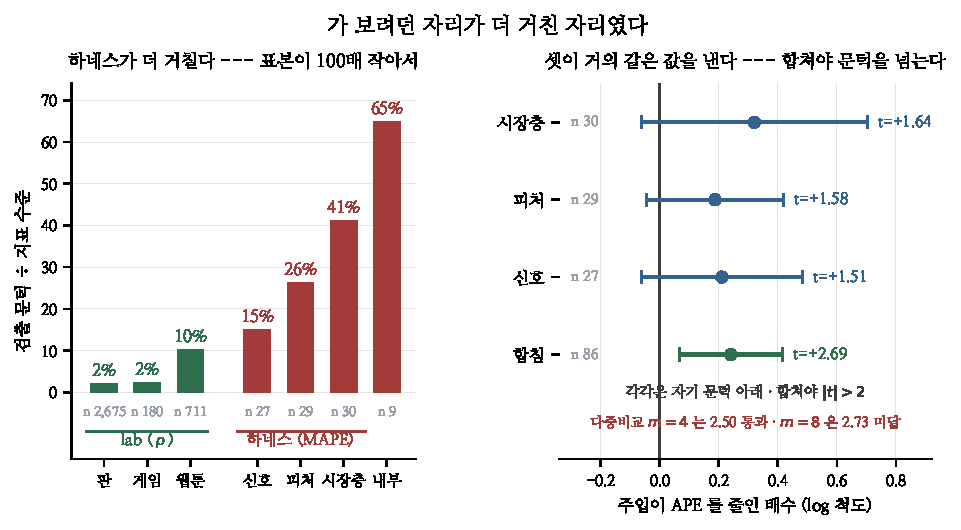
\includegraphics[width=\textwidth]{figs/floor.pdf}
\caption{왼쪽 --- 지표 수준으로 나눈 검출 문턱. 오른쪽 --- 배수 척도로 다시
잰 세 주입 효과와 합친 것($\pm$1.96\,짝SE).}
\end{figure*}

노트 274의 법칙을 그대로 적용했다.

\begin{center}\footnotesize
\begin{tabular}{lrrrr}
\hline
자리 & 수준 & 문턱 & 비 & 유보 $n$ \\
\hline
lab 판 & 0.4819 & 0.0100 & \textbf{2\%} & 2,675 \\
lab 게임 & 0.6158 & 0.0150 & \textbf{2\%} & 180 \\
lab 웹툰 & 0.4500 & 0.0460 & 10\% & 711 \\
\hline
하네스 신호 & 1.4930 & 0.2245 & 15\% & 27 \\
하네스 피처 & 1.4420 & 0.3808 & 26\% & 29 \\
하네스 시장층 & 0.7289 & 0.3004 & 41\% & 30 \\
\textbf{하네스 내부} & 0.1890 & 0.1227 & \textbf{65\%} & \textbf{9} \\
\hline
\end{tabular}
\end{center}

\textbf{하네스가 더 거칠다.} 그리고 \textbf{제일 거친 것이 내부 폴드}다 ---
라벨이 실측이라 MAPE 가 0.19 로 낮은 그 폴드가, 레코드 9건에 실행 잡음이
0.13 이라 짝 A/B 를 한 번씩 돌리면 문턱이 \textbf{수준의 65\%}다. 내가 세
노트에서 인용한 ``MAPE 16$\sim$18\%''가 바로 이 폴드다. \textbf{제일 좋아
보이는 숫자가 제일 못 재는 자리에서 나왔다.}

\paragraph{원인은 표본이다} lab 은 유보 2,675행을 채점한다. 하네스는 A/B 당
27$\sim$30건이다 --- \textbf{100배}다. 게다가 APE 짝차가 두꺼운 꼬리를 가진다:
절대값 상위 3건이 총합의 \textbf{52 · 71 · 53\%}를 차지한다(최대 5.40).

\paragraph{그래서 세 보고가 전부 문턱 아래다}

\begin{center}\small
\begin{tabular}{lrrr}
\hline
& 효과 & 문턱 & $t$ \\
\hline
시장층 & $+$0.0788 & 0.3004 & $+$0.52 \\
피처 & $+$0.2034 & 0.3808 & $+$1.07 \\
신호 & $+$0.1957 & 0.2245 & $+$1.74 \\
\hline
\end{tabular}
\end{center}

\section{척도를 바꾸니 셋이 같은 말을 한다}

여기서 멈추면 ``하네스도 아무것도 못 잰다''로 끝난다. 갈랐다(노트 133).

\textbf{APE 는 이미 비율이다.} 0.07 $\to$ 0.05 와 2.9 $\to$ 2.7 을 같은
$-$0.2 로 세는 것이 척도의 잘못이다. 비로 다시 쟀다
($\log\frac{\text{뺀 팔}+0.05}{\text{넣은 팔}+0.05}$).

\begin{center}\small
\begin{tabular}{lrrrr}
\hline
& $n$ & 효과 & $t$ & 필요 $n$ \\
\hline
시장층 & 30 & $+$0.3204 & $+$1.64 & 45 \\
피처 & 29 & $+$0.1874 & $+$1.58 & 46 \\
신호 & 27 & $+$0.2107 & $+$1.51 & 47 \\
\hline
\textbf{합침} & \textbf{86} & \textbf{$+$0.2411} & \textbf{$+$2.69} & --- \\
\hline
\end{tabular}
\end{center}

\textbf{$t$ 가 1.64 · 1.58 · 1.51 이다.} 서로 레코드가 안 겹치고 뺀 것도
다른 세 실험이 거의 같은 값을 낸다. 더하기 척도에서는 0.52 $\sim$ 1.74 로
흩어져 있던 것이다 --- \textbf{척도가 맞으면 잡음이 줄고 일치가 보인다.}

합치면 $n{=}86$ 에 $t{=}+2.69$, 되돌리면 \textbf{주입이 APE 를 21.4\% 줄인다.}

\paragraph{그런데 넘었다고 말하지 않는다} 노트 275의 배포 규칙대로 다중비교
문턱을 건다. 척도를 둘 봤고 비교를 넷 했다.

\begin{center}\small
\begin{tabular}{lrl}
\hline
셈 & 문턱 & $t{=}2.69$ \\
\hline
단일 ($m{=}1$) & 1.96 & 통과 \\
셋 $+$ 합침 ($m{=}4$) & 2.50 & 통과 \\
$\times$ 두 척도 ($m{=}8$) & \textbf{2.73} & \textbf{미달} \\
\hline
\end{tabular}
\end{center}

\textbf{내가 척도를 고른 것이 자료를 본 뒤다.} 그러니 $m{=}8$ 이 정직한
셈이고, 그 문턱을 0.04 차이로 못 넘는다. \textbf{``넘었다''가 아니라
``넘기 직전''이다.}

\section{갈 곳이 아니라 넓힐 곳이었다}

필요 표본이 셋 다 \textbf{45$\sim$47건}인데 지금 27$\sim$30건이다. 그리고

\begin{center}\small
\begin{tabular}{lr}
\hline
라벨 있는 시장 레코드 & 205 \\
세 A/B 가 쓴 것 & 86 \\
\textbf{아직 안 쓴 것} & \textbf{120} \\
\hline
\end{tabular}
\end{center}

\textbf{각 셋에 15$\sim$20건씩만 더하면 셋 다 자기 힘으로 문턱을 넘는다.}
그러면 척도 선택도 자료를 보기 전에 고정할 수 있어 $m{=}8$ 이 아니라
$m{=}3$ 이 된다.

\paragraph{남은 것}
\begin{center}\small
\begin{tabular}{ll}
\hline
갈래 & 왜 \\
\hline
셋에 20건씩 더 & 문턱을 각자 넘게. 라벨 120건 남음 \\
척도를 먼저 고정 & 배수. 다음 재기 전에 적어 둔다 \\
내부 폴드 앙상블 & 실행 잡음 0.13 이 문턱의 전부 \\
lab 회사 축 & 노트 294의 $+$0.0040 을 남길지 \\
\hline
\end{tabular}
\end{center}

\paragraph{규약} \textbf{``저기가 낫다''고 세 번 적기 전에 한 번 재라.}
하네스는 lab 이 못 재는 것을 재 주는 자리가 아니라 \textbf{더 못 재는
자리}였고, 재료는 처음부터 디스크에 있었다. 그리고 \textbf{척도를 자료 보고
고르면 그 값으로 다중비교를 물어야 한다} --- 배수 척도가 옳다고 지금은
믿지만, 그 믿음이 자료 뒤에 생겼으므로 이번 $t{=}2.69$ 는 증거가 아니라
\textbf{다음 측정의 설계}다.

\end{document}
